% The four memory organisations around the same core. Build: tectonic systems.tex
\documentclass[tikz,border=3pt]{standalone}
\usepackage[T1]{fontenc}
\usepackage{mathptmx}
\usetikzlibrary{arrows.meta}
\definecolor{ipath}{HTML}{2A78D6}
\definecolor{dpath}{HTML}{EB6834}
\definecolor{ink2}{HTML}{52514E}
\begin{document}
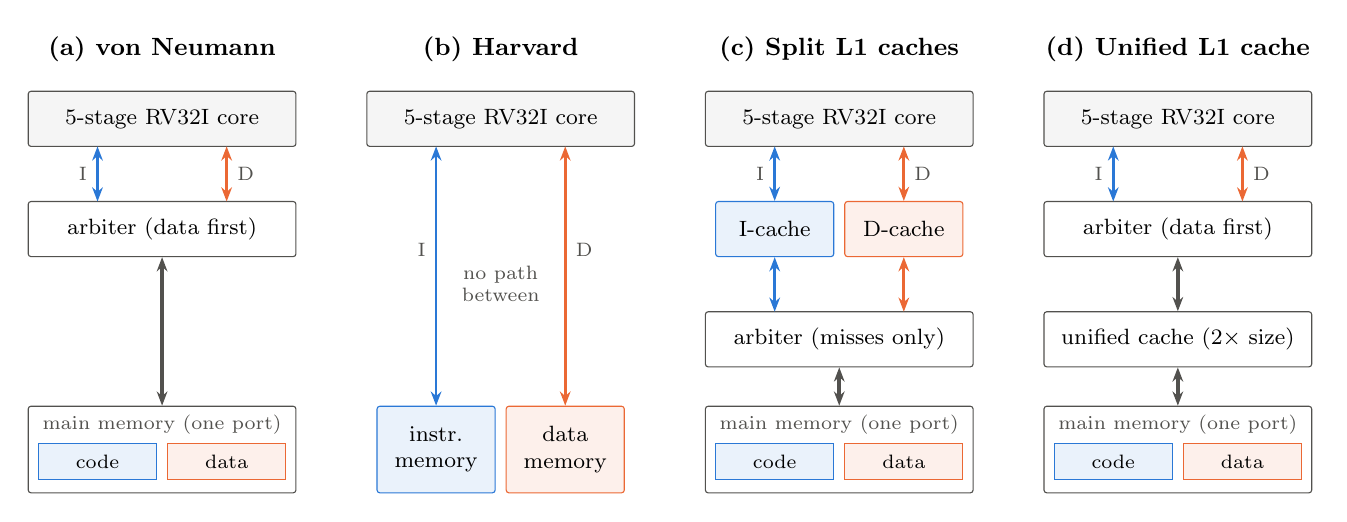
\begin{tikzpicture}[
    font=\footnotesize,
    blk/.style={draw=ink2, rounded corners=1pt, minimum height=7mm, align=center, fill=white},
    core/.style={blk, minimum width=34mm, fill=black!4},
    ibox/.style={blk, draw=ipath, fill=ipath!10, minimum width=15mm},
    dbox/.style={blk, draw=dpath, fill=dpath!10, minimum width=15mm},
    sbox/.style={blk, minimum width=34mm},
    ibus/.style={{Stealth[length=1.8mm]}-{Stealth[length=1.8mm]}, draw=ipath, line width=1pt},
    dbus/.style={{Stealth[length=1.8mm]}-{Stealth[length=1.8mm]}, draw=dpath, line width=1pt},
    shared/.style={{Stealth[length=1.8mm]}-{Stealth[length=1.8mm]}, draw=ink2, line width=1.5pt},
    title/.style={font=\small\bfseries, anchor=south},
    lbl/.style={font=\scriptsize, text=ink2},
]
    % Main memory, drawn the same way in every panel: code half and data half
    \newcommand{\mainmemory}[1]{
        \node[sbox, minimum height=11mm] (#1mem) at (0, 0.2) {};
        \node[lbl, anchor=north] at (#1mem.north) {main memory (one port)};
        \node[draw=ipath, fill=ipath!10, minimum width=15mm, minimum height=4.5mm, font=\scriptsize] at (-0.82, 0.05) {code};
        \node[draw=dpath, fill=dpath!10, minimum width=15mm, minimum height=4.5mm, font=\scriptsize] at (0.82, 0.05) {data};
    }

    % (a) von Neumann
    \begin{scope}[xshift=0cm]
        \node[title] at (0, 5.0) {(a) von Neumann};
        \node[core] (a_core) at (0, 4.4) {5-stage RV32I core};
        \node[sbox] (a_arb) at (0, 3.0) {arbiter (data first)};
        \mainmemory{a_}
        \draw[ibus] (-0.82, 4.05) -- node[lbl, left] {I} (-0.82, 3.35);
        \draw[dbus] (0.82, 4.05) -- node[lbl, right] {D} (0.82, 3.35);
        \draw[shared] (a_arb) -- (a_mem.north);
    \end{scope}

    % (b) Harvard
    \begin{scope}[xshift=4.3cm]
        \node[title] at (0, 5.0) {(b) Harvard};
        \node[core] (b_core) at (0, 4.4) {5-stage RV32I core};
        \node[ibox, minimum height=11mm] (b_imem) at (-0.82, 0.2) {instr.\\memory};
        \node[dbox, minimum height=11mm] (b_dmem) at (0.82, 0.2) {data\\memory};
        \draw[ibus] (-0.82, 4.05) -- node[lbl, left, pos=0.4] {I} (b_imem.north);
        \draw[dbus] (0.82, 4.05) -- node[lbl, right, pos=0.4] {D} (b_dmem.north);
        \node[lbl, align=center] at (0, 2.3) {no path\\between};
    \end{scope}

    % (c) Split L1 caches over one main memory (modified Harvard)
    \begin{scope}[xshift=8.6cm]
        \node[title] at (0, 5.0) {(c) Split L1 caches};
        \node[core] (c_core) at (0, 4.4) {5-stage RV32I core};
        \node[ibox] (c_ic) at (-0.82, 3.0) {I-cache};
        \node[dbox] (c_dc) at (0.82, 3.0) {D-cache};
        \node[sbox] (c_arb) at (0, 1.6) {arbiter (misses only)};
        \mainmemory{c_}
        \draw[ibus] (-0.82, 4.05) -- node[lbl, left] {I} (c_ic.north);
        \draw[dbus] (0.82, 4.05) -- node[lbl, right] {D} (c_dc.north);
        \draw[ibus] (c_ic.south) -- (-0.82, 1.95);
        \draw[dbus] (c_dc.south) -- (0.82, 1.95);
        \draw[shared] (c_arb) -- (c_mem.north);
    \end{scope}

    % (d) Unified L1 cache
    \begin{scope}[xshift=12.9cm]
        \node[title] at (0, 5.0) {(d) Unified L1 cache};
        \node[core] (d_core) at (0, 4.4) {5-stage RV32I core};
        \node[sbox] (d_arb) at (0, 3.0) {arbiter (data first)};
        \node[sbox] (d_cache) at (0, 1.6) {unified cache (2$\times$ size)};
        \mainmemory{d_}
        \draw[ibus] (-0.82, 4.05) -- node[lbl, left] {I} (-0.82, 3.35);
        \draw[dbus] (0.82, 4.05) -- node[lbl, right] {D} (0.82, 3.35);
        \draw[shared] (d_arb) -- (d_cache);
        \draw[shared] (d_cache) -- (d_mem.north);
    \end{scope}
\end{tikzpicture}
\end{document}
